% !TEX TS-program = pdflatex
% !TEX encoding = UTF-8 Unicode

% This is a simple template for a LaTeX document using the "article" class.
% See "book", "report", "letter" for other types of document.

\documentclass[12pt]{article} % use larger type; default would be 10pt
\usepackage[fontsize=12pt]{fontsize}
\renewcommand{\baselinestretch}{1.5} % linespacing=1.5
\usepackage[T2A]{fontenc} % кодировка
\usepackage{fontspec} % for changing fonts 
% \setmainfont{Times New Roman}
\setmainfont{Minion Pro}
% \setmainfont{Roboto}
% \usepackage[utf8]{inputenc} % set input encoding (not needed with XeLaTeX)
\usepackage[english]{babel} % for cyrillic letters support
\usepackage[parfill]{parskip} % remove space vefore parapraph
\setlength{\parskip}{0pt} % additional skip between paragraphs


%%% PAGE DIMENSIONS
\usepackage{geometry} % to change the page dimensions
\geometry{a4paper} % or letterpaper (US) or a5paper or....
\geometry{left=30mm,right=20mm,top=15mm, bottom=15mm} % for example, change the margins to 2 inches all round
% \graphicspath{{./images/}}
% \geometry{landscape} % set up the page for landscape
%   read geometry.pdf for detailed page layout information

\usepackage{graphicx} % support the \includegraphics command and options

% \usepackage[parfill]{parskip} % Activate to begin paragraphs with an empty line rather than an indent

%%% PACKAGES
\usepackage{blindtext}
\usepackage{booktabs} % for much better looking tables
\usepackage{multirow}
\usepackage{array} % for better arrays (eg matrices) in maths
\usepackage{paralist} % very flexible & customisable lists (eg. enumerate/itemize, etc.)
\usepackage{verbatim} % adds environment for commenting out blocks of text & for better verbatim
\usepackage{subfig} % make it possible to include more than one captioned figure/table in a single float
\usepackage{cmap} % search in pdf
\usepackage{longtable} % for long tables 
\usepackage{lscape}
\usepackage{hyperref} % for hyperlinks
\usepackage{listings} % for code listings
% These packages are all incorporated in the memoir class to one degree or another...

%% Useful packages
\usepackage[colorinlistoftodos]{todonotes}
% \usepackage[colorlinks=true, allcolors=blue]{hyperref}



\usepackage{amsmath,amsthm,amsfonts,amssymb,amscd, fancyhdr, color, comment, graphicx, environ}
\usepackage{float}
\usepackage{mathrsfs}
\usepackage[math-style=ISO]{unicode-math}
\setmathfont{TeX Gyre Termes Math}
\setmonofont{Hack Nerd Font Mono}
\usepackage{lastpage}
\usepackage[dvipsnames]{xcolor}
% \usepackage[framemethod=TikZ]{mdframed}
\usepackage{indentfirst}
\usepackage{thmtools}
\usepackage{shadethm}
\usepackage{setspace}


\definecolor{codegreen}{rgb}{0,0.6,0}
\definecolor{codegray}{rgb}{0.5,0.5,0.5}
\definecolor{codepurple}{rgb}{0.58,0,0.82}
\definecolor{backcolour}{rgb}{0.95,0.95,0.92}


%%% HEADERS & FOOTERS
\usepackage{fancyhdr} % This should be set AFTER setting up the page geometry
\pagestyle{fancy} % options: empty , plain , fancy
\renewcommand{\headrulewidth}{0pt} % customise the layout...
\lhead{}\chead{}\rhead{}
\lfoot{}\cfoot{\thepage}\rfoot{}

%%% SECTION TITLE APPEARANCE
\usepackage{titlesec}
\usepackage{sectsty}
\sectionfont{\centering}
\subsectionfont{\centering}

\usepackage{enumitem}
\setlist{nolistsep}

\hypersetup{
    colorlinks=true,
    linkcolor=black,
    filecolor=magenta,      
    urlcolor=blue,
    pdftitle={Overleaf Example},
    pdfpagemode=FullScreen,
    }
\urlstyle{same}




\lstdefinestyle{mystyle}{
    extendedchars=\true,
    inputencoding=utf8x,
    backgroundcolor=\color{backcolour},   
    commentstyle=\color{codegreen},
    keywordstyle=\color{magenta},
    numberstyle=\tiny\color{codegray},
    stringstyle=\color{codepurple},
    basicstyle=\ttfamily\footnotesize,
    breakatwhitespace=false,         
    breaklines=true,                 
    captionpos=b,                    
    keepspaces=true,                 
    numbers=left,                    
    numbersep=5pt,                  
    showspaces=false,                
    showstringspaces=false,
    showtabs=false,                  
    tabsize=2
}

\lstset{style=mystyle}




% \allsectionsfont{\sffamily\mdseries\upshape} % (See the fntguide.pdf for font help)
% (This matches ConTeXt defaults)

%%% ToC (table of contents) APPEARANCE
% \usepackage[nottoc,notlof,notlot]{tocbibind} % Put the bibliography in the ToC
% \usepackage[titles,subfigure]{tocloft} % Alter the style of the Table of Contents
% \renewcommand{\cftsecfont}{\rmfamily\mdseries\upshape}
% \renewcommand{\cftsecpagefont}{\rmfamily\mdseries\upshape} % No bold!
\makeatletter
\renewcommand{\fnum@figure}{Picture. \thefigure}
\makeatother



\renewcommand\lstlistingname{Algorithm}
\renewcommand\lstlistlistingname{Algorithms}
\def\lstlistingautorefname{Alg.}

\title{Market place Course Work}

\author{Baktybekov.N, Manurov.A, Erkin}

\begin{document}

\maketitle

\newpage
\tableofcontents{}
\setcounter{page}{1}

\newpage
\addcontentsline{toc}{section}{Введение}

    %1. Введение. В этом разделе описывается цель проекта и основные принципы, на которых он основан.
     
    %2. Описание функциональности. В этом разделе описываются функции, которые должны быть реализованы в проекте. Каждая функция должна быть описана подробно, с указанием ее цели и основных требований.
     
    %3. Архитектура проекта. В этом разделе описывается архитектура проекта, то есть как он устроен внутри. Это включает в себя описание используемых технологий, структуру базы данных и API.
     
    %4. Дизайн интерфейса. В этом разделе описывается дизайн пользовательского интерфейса, включая макеты и функциональные элементы.
     
    %5. Развертывание и использование. В этом разделе описывается процесс развертывания проекта и его использование. Он должен включать в себя инструкции по установке и настройке, а также рекомендации по использованию.
     
    %6. Тестирование. В этом разделе описывается процесс тестирования проекта. Он должен включать в себя описание методологии тестирования, список тестовых сценариев и результаты тестирования.
     
    %7. Сопровождение и поддержка. В этом разделе описываются процессы сопровождения и поддержки проекта после его внедрения. Он должен включать в себя инструкции по обслуживанию проекта, обновлениям и исправлению ошибок.

\section*{Введение}

\textbf{Ввод в экскурс}


Маркетплейсы в привычном для нас понимании существовали практически всю историю с момента зарождения человечества. С развитием науки и техники маркетплейсы также развивались становясь все удобнее и доступнее.
С изобретением компьютера и последующей компьютеризацией маркетплейсы трансформировались и перебрались в интернет пространство.
На данный момент существует тысячи интернет платформ маркетплейсов предоставляющих доступные способы размещения и просматривания товаров и услуг таких как Avito, Lalafo, Bazar.kg, Kerek.kg  и т.д. 

\textbf{Цель этого проекта} - создание маркетплейса, аналогичного Avito, используя язык программирования Java и фреймворк Spring. В этой документации будет обзор существующих решений на рынке, функции, которыми должен обладать сайт, и то, чем он может быть лучше существующих решений.
Обзор существующих решений на рынке



\section{Исследование предметной области}
\subsection{Обзор существующих решений на рынке}


На рынке существует множество маркетплейсов, таких как Amazon, eBay, Etsy и Avito. Каждый из них имеет свои функции и особенности.

% \bigbreak
% \bigbreak

\textbf{Amazon}

\begin{figure}[h]
    \centering
    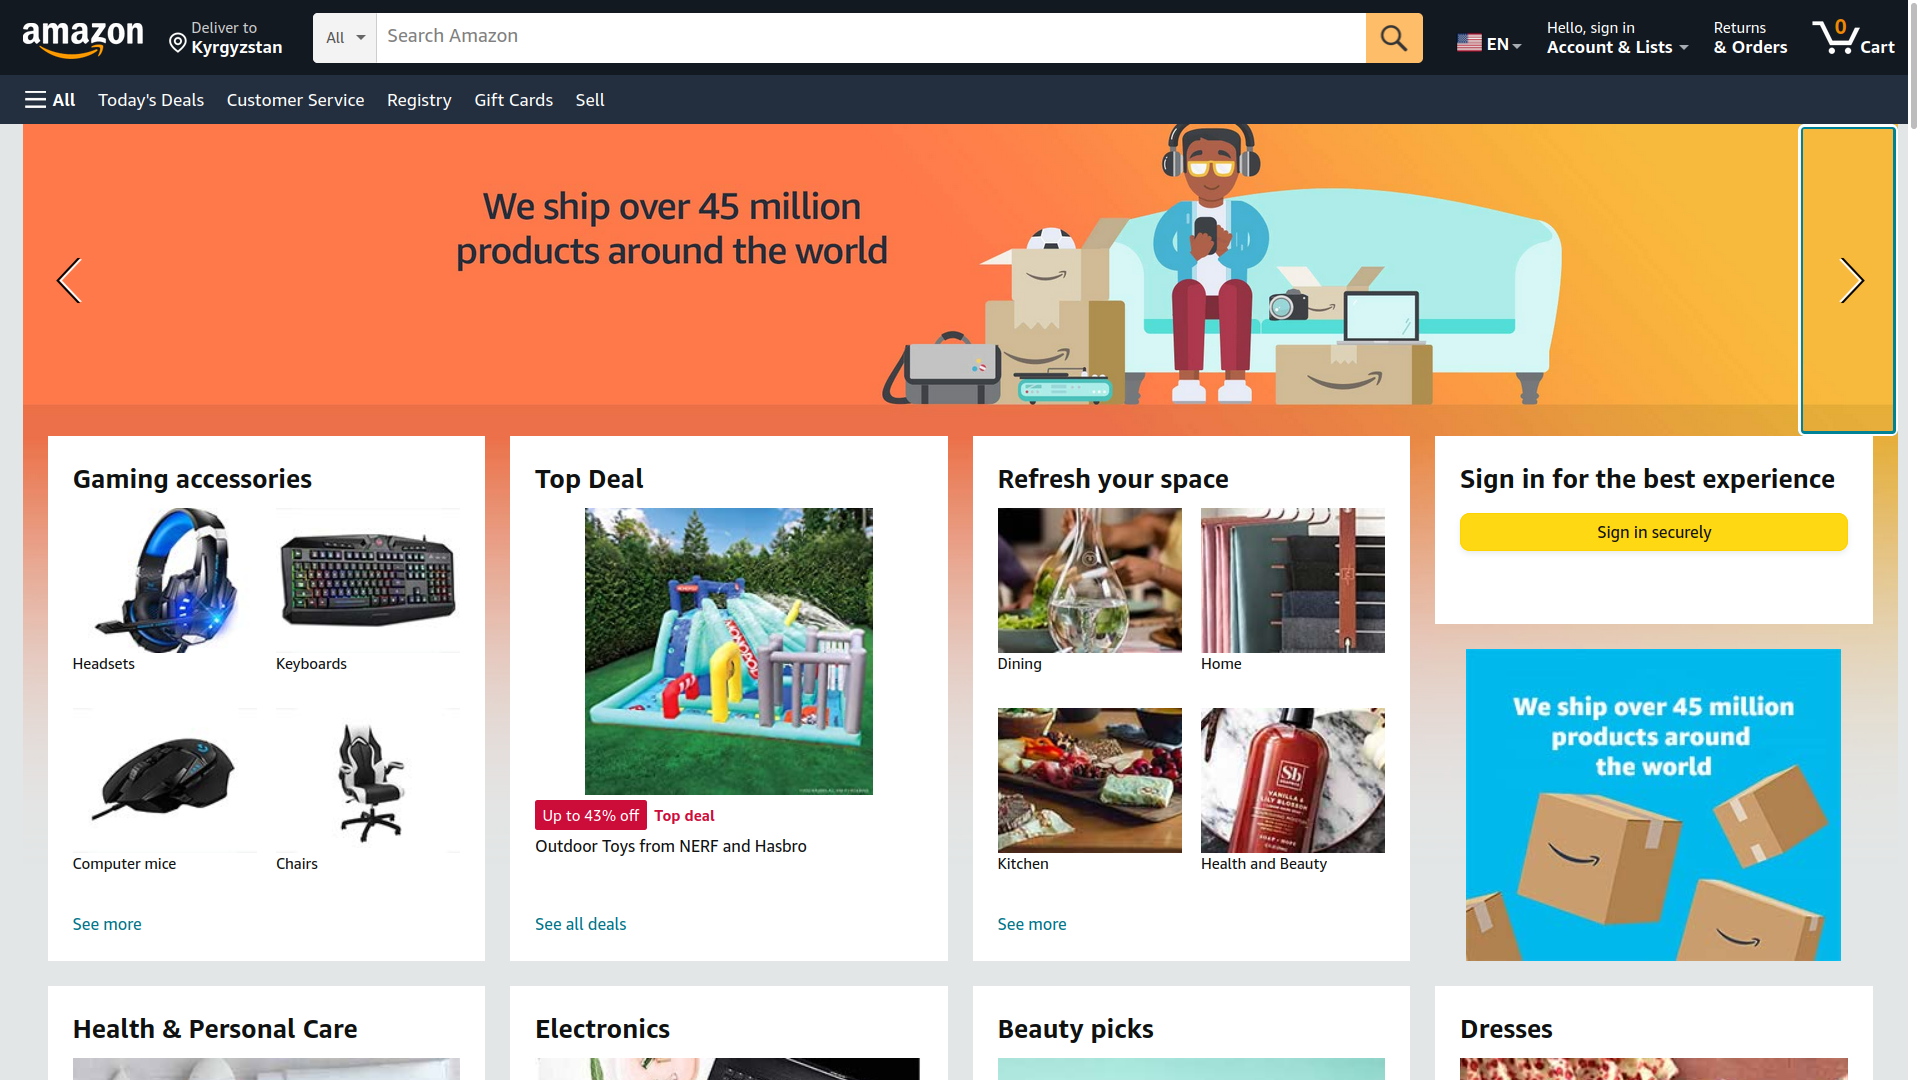
\includegraphics[width=0.8\textwidth]{./images/amazon_main.png}
    \caption{Amazon page}
\end{figure}

Amazon - это один из самых крупных онлайн-маркетплейсов в мире. Рассмотрим подробнее его функции, достоинства и недостатки:

\textbf{\emph{Функции:}}

% {\setlength{\leftmargini}{1pt}
\begin{compactitem}
    \item  Широкий ассортимент товаров: Amazon предлагает огромный выбор товаров во многих категориях, включая электронику, одежду, книги, продукты питания и многое другое.

    \item  Быстрая доставка: Amazon предлагает быструю доставку по всему миру, что позволяет покупателям получать свои товары в кратчайшие сроки.

    \item  Персонализированный опыт покупки: Amazon использует данные о покупателе и его предпочтениях, чтобы предложить наиболее релевантные товары и рекомендации.

    \item Amazon Prime: подписчики Amazon Prime получают бесплатную доставку на многие товары, доступ к потоковому видео и многим другим преимуществам.

    \item  Amazon Web Services: Amazon предлагает облачные сервисы для бизнеса, включая хранение данных, обработку и аналитику, что делает его одним из крупнейших провайдеров облачных услуг.
\end{compactitem}

\textbf{\emph{Достоинства:}}

\begin{compactitem}
    \item  Широкий ассортимент товаров: благодаря огромному выбору товаров, Amazon является одним из лидеров на рынке онлайн-маркетплейсов.

    \item  Высокое качество обслуживания: Amazon имеет высокую репутацию в области обслуживания клиентов, предлагая быструю и эффективную помощь при возникновении проблем.

    \item  Быстрая доставка: благодаря своей разветвленной системе логистики, Amazon предлагает быструю доставку в большинстве регионов мира.

    \item  Amazon Prime: подписчики Amazon Prime получают доступ к эксклюзивным акциям и специальным предложениям, а также бесплатной доставке на многие товары.

    \item  Amazon Web Services: сервисы облачных вычислений Amazon Web Services используются многими компаниями по всему миру, что позволяет им быстро масштабировать свой бизнес и уменьшить затраты на инфраструктуру.
\end{compactitem}

\textbf{\emph{Недостатки:}}

\begin{compactitem}
    \item  Высокие комиссии: Amazon взимает высокие комиссии с продавцов, что может увеличить цену товаров для покупателей.

    \item  Конкуренция: из-за большого количества продавцов на платформе Amazon, конкуренция может быть слишком высокой, что может затруднить продажи для некоторых продавцов.

    \item  Политика возврата товаров: Amazon имеет строгую политику возврата товаров, которая может быть неудобной для некоторых покупателей.

    \item  Зависимость от логистических компаний: Amazon полагается на сторонние логистические компании для доставки товаров, что может привести к проблемам с доставкой в некоторых регионах.

    \item  Контроль над продавцами: Amazon имеет полный контроль над продавцами на своей платформе, что может привести к недостатку свободы для продавцов в установлении собственных правил и цен.
\end{compactitem}

В целом, Amazon является одним из самых крупных и популярных онлайн-маркетплейсов в мире. Он предлагает широкий ассортимент товаров, быструю доставку и персонализированный опыт покупки, а также имеет множество преимуществ для подписчиков Amazon Prime и бизнес-клиентов, использующих сервисы Amazon Web Services. Однако, существуют и некоторые недостатки, такие как высокие комиссии для продавцов, жесткая политика возврата товаров и зависимость от сторонних логистических компаний, что могут снизить удобство покупки для некоторых покупателей и продавцов.







\bigbreak
\bigbreak

\textbf{eBay}

\begin{figure}[h]
    \centering
    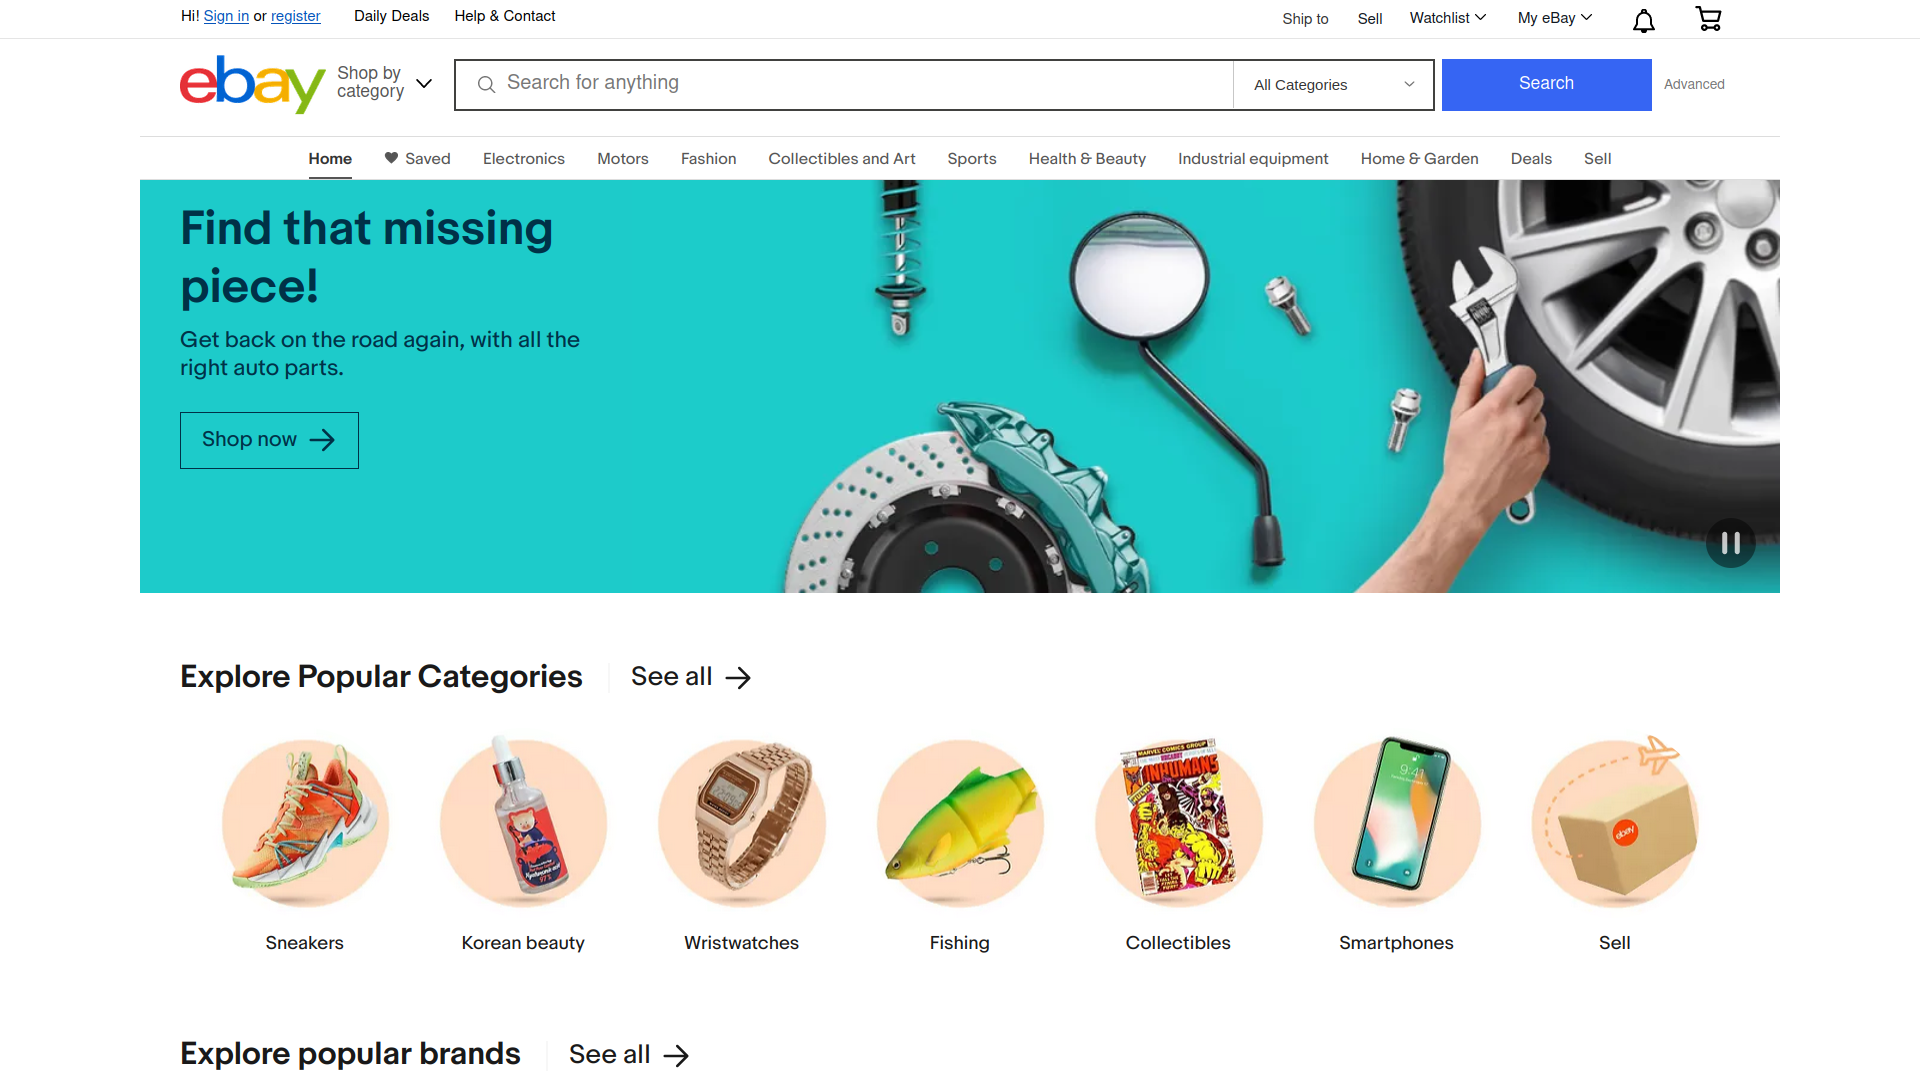
\includegraphics[width=0.8\textwidth]{./images/ebay_main.png}
    \caption{eBay main page}
\end{figure}


eBay - это еще один крупный онлайн-маркетплейс, предлагающий широкий ассортимент товаров, включая новые и б/у товары, аукционы и немедленные покупки. Вот подробный обзор и анализ функций, достоинств и недостатков eBay с вашей точки зрения:

\textbf{\emph{Функции:}}

\begin{compactitem}
    \item  Аукцион: eBay предлагает уникальную функцию аукциона, которая позволяет покупателям участвовать в торгах за товары и получить их по лучшей цене.

    \item  Немедленная покупка: наряду с аукционами, eBay также предлагает возможность немедленной покупки товаров по фиксированной цене.

    \item  Широкий ассортимент: eBay предлагает огромный выбор товаров, включая редкие и уникальные товары, которые можно найти только на этой платформе.

    \item  Мировая доставка: eBay предоставляет возможность мировой доставки товаров, что делает покупки на платформе более доступными для покупателей из разных стран.

    \item  Защита покупателя: eBay имеет политику защиты покупателей, которая обеспечивает возмещение покупателям, если они получают товар, который не соответствует описанию или не был доставлен.
\end{compactitem}

\textbf{\emph{Достоинства:}}

\begin{compactitem}
    \item  Широкий выбор товаров: eBay предлагает огромный выбор товаров, включая редкие и уникальные, которые трудно найти на других платформах.

    \item  Гибкость цен: eBay позволяет продавцам устанавливать цены на свои товары, что дает им большую гибкость в управлении своим бизнесом.

    \item  Доступность для малых бизнесов: eBay может быть хорошим выбором для малых бизнесов, которые хотят начать продавать товары онлайн, так как он предлагает относительно низкие комиссии для продавцов.

    \item  Быстрая доставка: eBay имеет свою собственную службу доставки, что может ускорить процесс доставки товаров.
\end{compactitem}

\textbf{\emph{Недостатки:}}

\begin{compactitem}
    \item  Конкуренция: конкуренция на платформе может быть высокой, что может затруднить продажи для некоторых продавцов.

    \item  Высокие комиссии: eBay взимает высокие комиссии с продавцов, что может сни

    \item  Сложности с возвратами: политика возвратов на eBay может быть сложной и не всегда защищает продавцов.

    \item  Риски мошенничества: на eBay может быть высокий риск мошенничества, поскольку продавцы и покупатели не всегда могут быть легко проверены.

    \item  Качество товаров: поскольку на eBay можно купить б/у товары, качество товаров может быть непредсказуемым и варьироваться от продавца к продавцу.
\end{compactitem}

\textbf{\emph{Сравнительный анализ:}}

eBay имеет сходства с Amazon в том, что он предлагает широкий выбор товаров и доставку во многие страны мира. Однако, eBay имеет более гибкие цены и более низкие комиссии для продавцов, что делает его более доступным для малых бизнесов. Также eBay предоставляет уникальную возможность участия в аукционах, которую Amazon не предлагает.

Однако, eBay имеет некоторые недостатки, которых нет у Amazon, такие как сложности с возвратами и высокий риск мошенничества. Кроме того, на eBay качество товаров может быть непредсказуемым и варьироваться от продавца к продавцу, в то время как на Amazon качество товаров обычно более предсказуемо.

В целом, eBay может быть хорошим выбором для покупателей, которые ищут редкие или уникальные товары, а также для продавцов, которые хотят начать продавать товары онлайн. Однако, его недостатки могут быть проблематичны для продавцов, которые ищут надежную платформу для продажи своих товаров.












\bigbreak
\bigbreak

\textbf{Etsy}

\begin{figure}[h]
    \centering
    
\includegraphics[width=0.8\textwidth]{./images/etsy_main.png}
    \caption{Etsy main page}
\end{figure}


Etsy - это онлайн-маркетплейс для продажи и покупки товаров, которые производятся вручную или имеют отношение к ручной работе. Сайт основан в 2005 году и на данный момент является одним из лидеров в своей нише. Рассмотрим его функции, достоинства и недостатки:

\textbf{\emph{Функции:}}

\begin{compactitem}
    \item  Создание личной учетной записи продавца или покупателя;
    \item  Разделение товаров на категории и подкатегории;
    \item  Поиск товаров по ключевым словам, тегам, названию магазина и имени продавца;
    \item  Просмотр описания товара, фотографий, отзывов и рейтинга продавца;
    \item  Корзина для покупок и оформление заказа;
    \item  Система сообщений для общения между продавцом и покупателем;
    \item  Наличие приложения для смартфонов.
\end{compactitem}

\textbf{\emph{Достоинства}}:

\begin{compactitem}
    \item  Etsy специализируется на ручной работе, что позволяет продавцам и покупателям находить уникальные и качественные товары;
    \item  Сайт предоставляет ряд инструментов для продвижения товаров, таких как оптимизация ключевых слов и просмотр статистики продаж;
    \item  Есть возможность создания персонализированного магазина;
    \item  Удобный и простой интерфейс сайта;
    \item  Система отзывов и рейтинга продавцов помогает оценить надежность и качество продукции;
    \item  Наличие мобильного приложения позволяет удобно покупать и продавать товары через смартфон.
\end{compactitem}

\textbf{\emph{Недостатки:}}

\begin{compactitem}
    \item  Некоторые продавцы используют Etsy для продажи товаров, которые не отвечают требованиям ручной работы, что противоречит концепции сайта;
    \item  Etsy взимает комиссию за каждую продажу, что может быть неприятным для некоторых продавцов;
    \item  Из-за концепции сайта, многие товары могут быть дороже, чем аналоги на других маркетплейсах;
    \item  Иногда возникают проблемы с доставкой и возвратом товаров, особенно для международных покупателей.
\end{compactitem}






% \bigbreak
% \bigbreak

\textbf{Avito}

\begin{figure}[h]
    \centering
    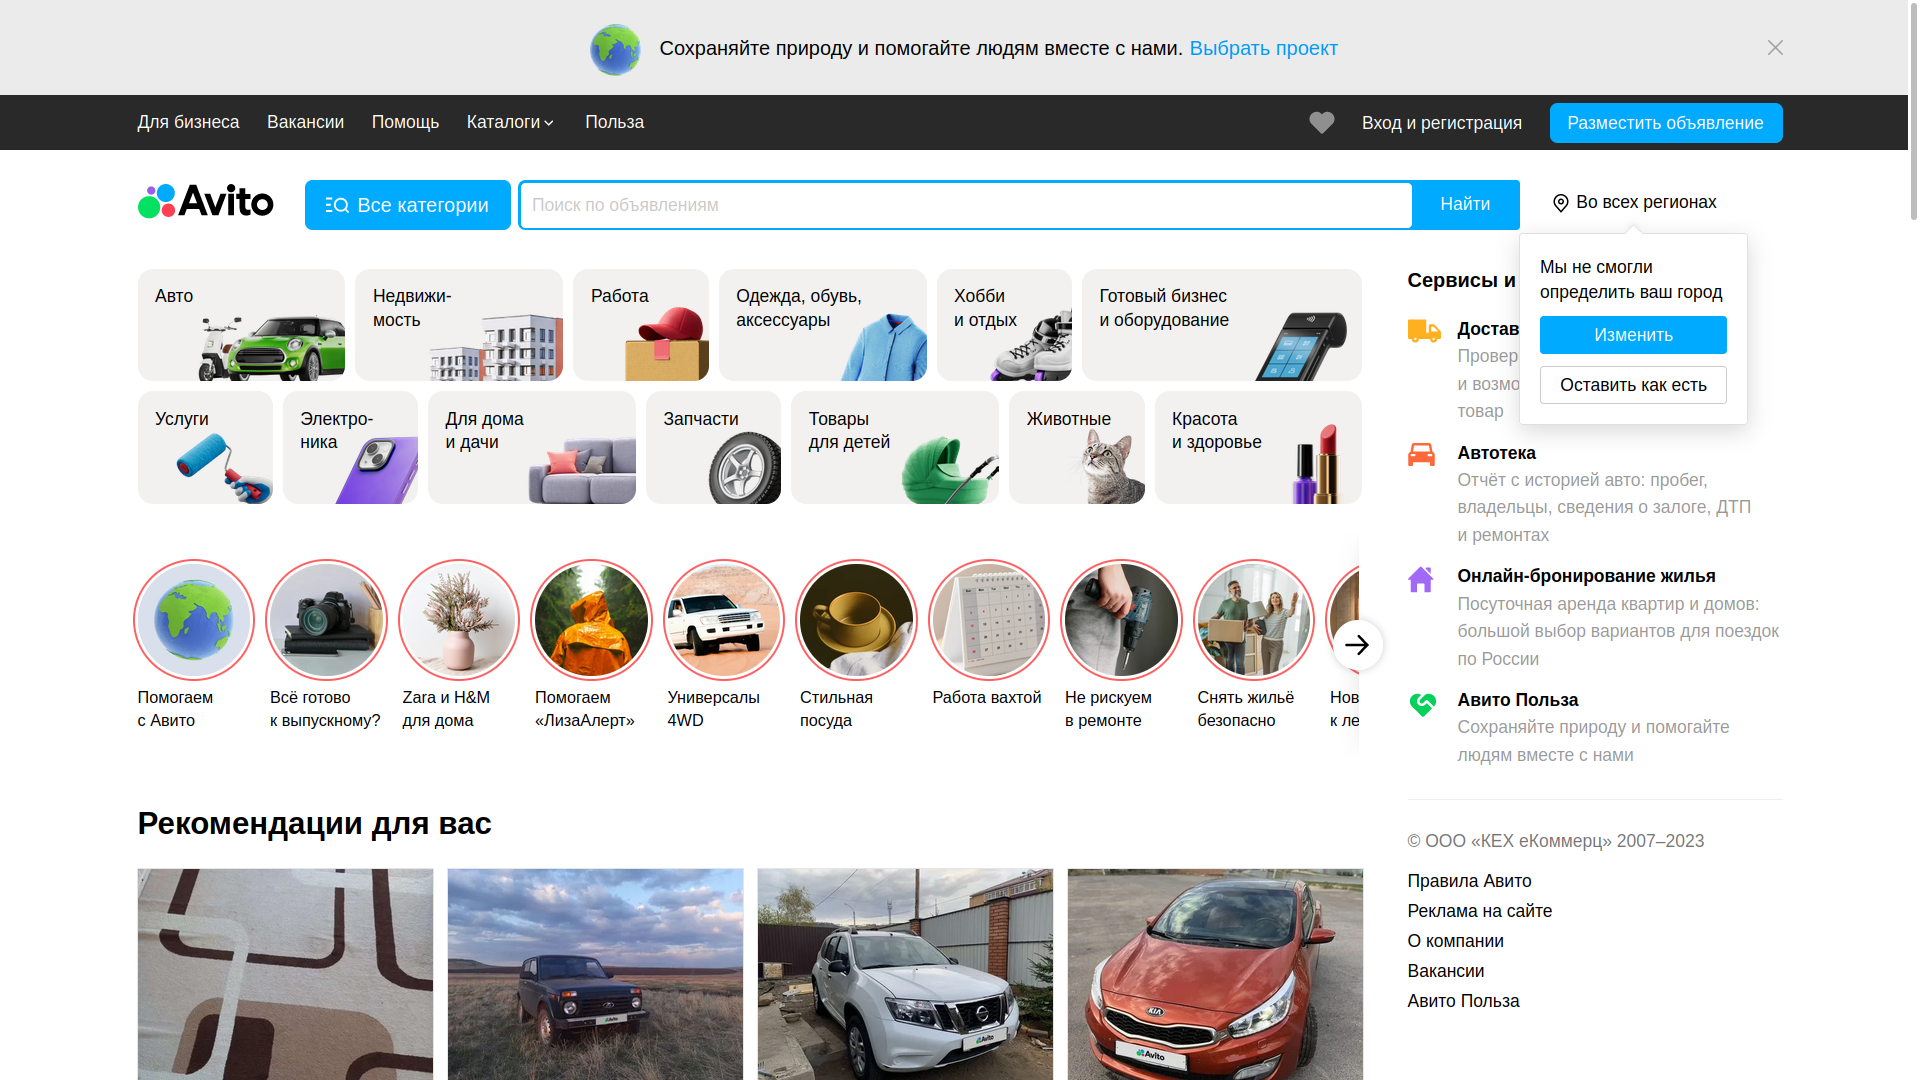
\includegraphics[width=0.8\textwidth]{./images/avito_main.png}
    \caption{Avito main page}
\end{figure}

Avito - это крупнейший российский онлайн-маркетплейс, на котором можно купить и продать различные товары и услуги. Рассмотрим его функции, достоинства и недостатки:

\textbf{\emph{Функции:}}

\begin{compactitem}
    \item  Создание личной учетной записи продавца или покупателя;
    \item  Разделение товаров на категории и подкатегории;
    \item  Поиск товаров по ключевым словам, фильтрам и регионам;
    \item  Просмотр описания товара, фотографий, контактной информации продавца и отзывов;
    \item  Корзина для покупок и оформление заказа;
    \item  Система сообщений для общения между продавцом и покупателем;
    \item  Размещение объявлений о продаже товаров и услуг;
    \item  Наличие мобильного приложения.
\end{compactitem}

\textbf{\emph{Достоинства:}}

\begin{compactitem}
    \item  Avito является самым крупным и популярным маркетплейсом в России, что обеспечивает большой поток покупателей и продавцов;
    \item  Возможность размещения бесплатных объявлений, что делает маркетплейс доступным для всех;
    \item  Широкий ассортимент товаров и услуг;
    \item  Удобный и простой интерфейс сайта;
    \item  Возможность найти товары в своем регионе и сэкономить на доставке;
    \item  Наличие мобильного приложения позволяет удобно покупать и продавать товары через смартфон.
\end{compactitem}

\textbf{\emph{Недостатки:}}

\begin{compactitem}
    \item  Наличие множества мошенников и недобросовестных продавцов, что может привести к потере денег и получению некачественного товара;
    \item  Многие продавцы стараются продавать товары по завышенным ценам;
    \item  Avito не имеет возможности оплаты товаров через сайт, что может вызвать неудобства при оплате;
    \item  Комиссия за каждую продажу может быть высокой для некоторых продавцов;
    \item  Качество фотографий и описаний товаров может быть низким, что затрудняет выбор покупателей;
    \item  Нет системы рейтинга продавцов и отзывов на каждое объявление, что может снизить доверие к продавцу и качеству товара.
\end{compactitem}


Avito - это удобный и популярный маркетплейс, который позволяет покупать и продавать товары и услуги в России. Однако, на сайте присутствует большое количество рекламы
Кроме того, Avito сильно ограничивает своих пользователей в возможностях. Например, на сайте нельзя создать более одного аккаунта, иначе они могут быть заблокированы. Также, для некоторых категорий товаров существуют ограничения на количество объявлений, которые можно разместить.
В целом, можно сказать, что Avito является достаточно качественным и удобным сервисом для онлайн-продаж, который имеет ряд сильных сторон и некоторые недостатки. При разработке аналогичного сайта-маркетплейса на Java и Spring, следует учитывать достоинства и недостатки уже существующих решений и стараться предоставить пользователям максимально удобный и надежный сервис.







\textbf{Функции нашего сайта}
Для создания маркетплейса, подобного Avito, необходимо реализовать следующие функции:

\begin{compactitem}
    \item  Регистрация и аутентификация пользователей
    \item  Создание профилей пользователей
    \item  Размещение объявлений и управление ими
    \item  Поиск товаров и услуг по категориям и регионам
    \item  Отображение информации о товарах и услугах
    \item  Возможность связаться с продавцом через сайт
    \item  Оставление отзывов и рейтинга продавцов
    \item  Настраиваемые уведомления
\end{compactitem}



\bigbreak
\bigbreak

\textbf{Цель:}

Конечная цель проекта - создание функционального маркетплейса, который позволит пользователям размещать свои объявления о продаже товаров и услуг, а также искать и приобретать нужные им товары и услуги у других пользователей.

Этот проект позволит студенту лучше понять язык программирования Java и фреймворк Spring, а также научиться проектировать и разрабатывать веб-приложения. Создание маркетплейса также требует понимания основных принципов взаимодействия пользователей, управления данными и безопасности веб-приложений.

Поэтому, целью этого проекта является не только создание конечного продукта, но и получение опыта разработки веб-приложения, понимание принципов его работы и применение на практике основных знаний, полученных на предыдущих этапах обучения.













\section{Описание функциональности}
В данном проекте должны быть реализованы следующие функции:

\begin{enumerate}[wide, labelwidth=!, labelindent=0pt]
    \item Регистрация на сайте
    \item Лента объявлений
    \item Личный кабинет
\end{enumerate}




\subsection{Регистрация на сайте}
    \textbf{Форма регистрации:} на сайте должна быть форма, которую пользователи заполняют, чтобы создать свой профиль. Форма может включать такие поля, как имя, фамилия, адрес электронной почты и пароль. Для удобства пользователей можно предоставить возможность автоматической генерации пароля или использовать социальные сети для быстрой регистрации.

    \textbf{Аутентификация:} после заполнения формы регистрации пользователь должен подтвердить свою учетную запись, нажав на ссылку в электронном письме, которое ему было отправлено. Это гарантирует, что адрес электронной почты пользователя действительный и что пользователь действительно хочет создать свой профиль.

    \textbf{Персонализация профиля:} после подтверждения своего адреса электронной почты пользователь может получить доступ к своему профилю. Здесь он может добавить информацию о себе, например, фотографию, контактные данные, а также настройки профиля.

    \textbf{Безопасность:} для обеспечения безопасности пользователей регистрационная форма должна содержать проверку на роботов (reCAPTCHA), а также механизмы защиты от хакерских атак, таких как SQL-инъекции и XSS-атаки.

    \textbf{Восстановление пароля:} для того, чтобы пользователи могли восстановить свой пароль, если его забыли, на сайте должна быть реализована функция восстановления пароля. Пользователь должен ввести свой адрес электронной почты, на который будет отправлено письмо со ссылкой для восстановления пароля.

    \textbf{Уведомления:} после успешной регистрации пользователя можно уведомлять о новых предложениях, скидках, акциях и других новостях, чтобы пользователь мог быть в курсе последних обновлений.


\subsection{Лента объявлений}
    \textbf{Фильтрация объявлений:} Пользователи могут отфильтровать объявления по различным параметрам, таким как категория товара, цена, местоположение и т.д.

    \textbf{Сортировка объявлений:} Пользователи могут отсортировать объявления по различным параметрам, таким как дата добавления, цена и т.д.

    \textbf{Поиск объявлений:} Пользователи могут воспользоваться поиском, чтобы быстро найти нужные им объявления.

    \textbf{Просмотр объявлений:} Пользователи могут просмотреть детали объявления, такие как описание товара, фотографии, цена, контактные данные продавца и т.д.

    \textbf{Сохранение объявлений:} Пользователи могут сохранять объявления из ленты или поиска в личный раздел избранное, которое пользователь сможет потом просмотреть. 

    \textbf{Добавление объявлений:} Пользователи могут добавлять свои объявления в систему, указывая информацию о товаре, цене, фотографии и т.д.

    \textbf{Редактирование объявлений:} Пользователи могут редактировать свои объявления, чтобы изменить информацию о товаре или цене.

    \textbf{Удаление объявлений:} Пользователи могут удалить свои объявления из системы, если они больше не актуальны или проданы.

    Для удобства пользователей, лента объявлений должна быть понятной и простой в использовании. Она должна отображать только актуальные объявления и обеспечивать возможность быстрого поиска и фильтрации по категориям и другим параметрам. Также рекомендуется добавить возможность сортировки по популярности или релевантности, чтобы помочь пользователям быстрее найти нужные им товары или услуги.


\subsection{Личный кабинет}

    \textbf{Профиль пользователя:} Здесь пользователь может просмотреть и отредактировать свои личные данные, такие как имя, электронная почта, номер телефона, адрес и т.д. Также пользователь может загрузить фото профиля.

    \textbf{Мои объявления:} Эта функция позволяет пользователям просмотреть все их активные и неактивные объявления. Пользователи могут изменять и удалять свои объявления.

    \textbf{Избранное:} Эта функция позволяет пользователям сохранять объявления, которые им понравились, в отдельном списке. Также пользователи могут отслеживать изменения в объявлениях, которые им интересны.

    % \textbf{История заказов:} Здесь пользователь может просмотреть историю всех заказов, сделанных на сайте маркетплейса. Каждый заказ должен содержать информацию о товаре, цене, продавце и дате заказа.

    \textbf{Сообщения:} Эта функция позволяет пользователям общаться с другими пользователями сайта маркетплейса. Пользователи могут отправлять сообщения продавцам, задавать вопросы и обсуждать детали сделок.

    \textbf{Настройки:} Здесь пользователь может настроить уведомления от сайта, изменить пароль и настроить другие параметры учетной записи.

    \textbf{Выход из учетной записи:} Эта функция позволяет пользователям выйти из своей учетной записи на сайте маркетплейса.

    Личный кабинет должен быть легким в использовании и предоставлять интуитивно понятный интерфейс, чтобы пользователи могли быстро находить нужные функции и легко управлять своей учетной записью и объявлениями.














\section{Архитектура проекта}

\subsection{Серверная часть}
    \textbf{Клиент-серверная архитектура:} приложение состоит из двух частей - клиентской и серверной. Клиентская часть представляет собой веб-интерфейс для пользователей, а серверная часть отвечает за обработку запросов от клиентской части и взаимодействие с базой данных.

    \textbf{Архитектура MVC (Model-View-Controller):} модель отвечает за работу с базой данных и хранение данных, представление - за отображение информации пользователю (веб-страницы), а контроллер - за обработку запросов и управление данными между моделью и представлением.

    \textbf{Использование Spring Framework:} Spring предоставляет множество инструментов для реализации проектов на Java, включая инструменты для работы с базами данных, веб-разработки, безопасности и т.д. В проекте можно использовать Spring Boot для автоматической настройки и конфигурации приложения.

    \textbf{RESTful API:} API (Application Programming Interface) обеспечивает взаимодействие между клиентской и серверной частями приложения. Реализация RESTful API позволит использовать стандартные HTTP-методы для передачи данных между клиентом и сервером.

    \textbf{Использование базы данных:} для хранения данных маркетплейса будет используется реляционная база данных SQlite. В базе данных будут храниться информация о пользователях, объявлениях, заказах и т.д.

    \textbf{Использование системы контроля версий:} используется система контроля верси - Git, для управления кодом проекта и его версиями. Это позволяет отслеживать изменения в коде, возвращаться к предыдущим версиям и работать в команде над проектом.

    \textbf{Реализация тестирования:} для обеспечения требуемой функциональности и отладки кода.


\subsection{Клиентская часть}
    \textbf{Главная страница:} это первая страница, которую увидит пользователь при открытии сайта. На этой странице должны быть представлены основные функции сайта и возможности поиска.

    \textbf{Страницы категорий:} каждая категория должна иметь свою страницу с перечнем товаров в этой категории.

    \textbf{Страницы товаров:} каждый товар должен иметь свою страницу с подробным описанием и изображениями товара.

    \textbf{Личный кабинет пользователя:} это страница, где пользователь может редактировать свой профиль, просматривать свои объявления, сообщения и т.д.

    \textbf{Корзина:} это страница, где пользователь может просмотреть все товары, которые он добавил в корзину, изменить количество товаров и оформить заказ.

    \textbf{Формы:} на сайте должны быть различные формы для заполнения, например, для регистрации, добавления товара или связи с поддержкой.

    Клиентская часть должна быть реализована с помощью HTML, CSS и JavaScript.Клиентская часть работает в основном на мобильных устройствах, десктоп версия практически не нужна.













\newpage
\section{Дизайн интерфейса}


\subsection{Структура сайта}

\textbf{Главные разделы приложения}

\begin{compactitem}
    \item Авторизация
    \item Каталог товаров/услуг
        \begin{compactitem}
            \item Категории
                \begin{compactitem}
                    \item Страница товара/услуги
                \end{compactitem}
            \item Страница товара/услуги
        \end{compactitem}
        
    \item Профиль
        \begin{compactitem}
            \item Избранное
            \item Мои объявления 
            \item Редактировать профиль
            \item Выйти
        \end{compactitem}
        
\end{compactitem}



% Please add the following required packages to your document preamble:
% \usepackage{longtable}
% Note: It may be necessary to compile the document several times to get a multi-page table to line up properly
{\small
    \setlength\tabcolsep{1.4pt}
\begin{longtable}{lll}
\hline
\textbf{Раздел} & \textbf{Эдементы} & \textbf{Описание} \\ \hline
\endfirsthead
%
\endhead
%
\multicolumn{1}{|l|}{\textit{\textbf{Верхняя панель}}} &
  \multicolumn{1}{l|}{\begin{tabular}[c]{@{}l@{}}Иконка профиля\\ Иконка поиска\end{tabular}} &
  \multicolumn{1}{l|}{\begin{tabular}[c]{@{}l@{}}При нажатии на иконку профиля\\ a. Появляется меню со\\ следующими элементами:\\ i.\\ Мои заказы\\ 1. Открывает\\ страницы\\ “История\\ заказов”\\ ii.\\ Редактировать профиль\\ 1. Открывает\\ страницу\\ “Профиль”\\ iii.\\ Поддержка\\ 1. Открывает\\ страницу для\\ обратной связи\\ “Поддержка”\\ iv.\\ Выйти\\ 1. Выходит из поль\\ пользователя\\ приложения\\ 2. Открывается\\ страница\\ “Авторизация”\end{tabular}} \\ \hline
\multicolumn{1}{|l|}{\textit{\textbf{Каталог товаров}}} &
  \multicolumn{1}{l|}{\begin{tabular}[c]{@{}l@{}}Иконки разделов\\ Карточки с объявлениями\end{tabular}} &
  \multicolumn{1}{l|}{\begin{tabular}[c]{@{}l@{}}При нажатии на вкладку\\ “Рестораны” на странице\\ отображается список карточек\\ ресторанов\\ 1.1.\\ Карточка ресторана содержит:\\ 1.1.1.\\ Картинку ресторана\\ 1.1.2.\\ Название ресторана\\ 1.1.3.\\ Название кухни\\ 1.2.\\ При нажатии на карточку\\ ресторана\\ 1.2.1.\\ Открывается страница\\ Ресторана\\ 2.\\ При нажатии на вкладку\\ “Магазины” на странице\\ отображается список карточек\\ магазинов\\ 2.1.\\ Карточка магазина содержит:\\ 2.1.1.\\ Картинку магазина\\ 2.1.2.\\ Название магазина\\ 2.1.3.\\ Тип продукции\\ 2.2.\\ При нажатии на карточку\\ магазины\\ 2.2.1.\\ Открывается страница\\ магазина\end{tabular}} \\ \hline
\multicolumn{1}{|l|}{\textit{\textbf{Страница товара/услуги}}} &
  \multicolumn{1}{l|}{\begin{tabular}[c]{@{}l@{}}Заголовок:\\ Название\\ ресторана\\ 2. Картинка\\ 3. Иконка локации\\ 4. Заголовок:\\ “Меню”\\ 5. Список карточек\\ блюд\end{tabular}} &
  \multicolumn{1}{l|}{\begin{tabular}[c]{@{}l@{}}При нажатии на иконку локации,\\ открывается карта на телефоне в\\ приложении, которые предлагает\\ смартфон.\\ 2. Карточка содержит:\\ a. Картинку продукта\\ b. Название продукта\\ c. Текстовое поле с кнопками\\ увеличения/уменьшения\\ количества (+/-)\\ i.\\ После указания\\ количества продуктов,\\ этот продукт\\ добавляется в корзину\\ ii.\\ У иконки корзины будет\\ появлятся цифра с\\ количеством\\ добавленных продуктов\end{tabular}} \\ \hline
\end{longtable}}




\subsection{Требования к дизайну}







\end{document}
